\documentclass[a4paper,11pt]{article}
\usepackage{tikz}
\usepackage{pgfplots}
\pgfplotsset{compat=1.17}

\begin{document}

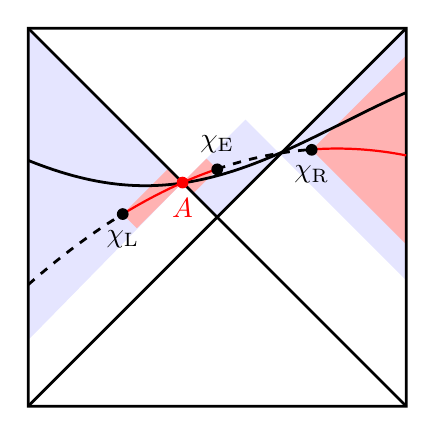
\begin{tikzpicture}[scale=0.8]
	\begin{scope}[transparency group]
			\path
			+(3,3)  coordinate (IItopright)
			+(-3,3) coordinate (IItopleft)
			+(3,-3) coordinate (IIbotright)
			+(-3,-3) coordinate(IIbotleft)

			;


			\fill[fill=blue!10] (-0.55,0.55) -- (0.45,1.55) -- (1,1) -- (0,0) -- cycle;

			\fill[fill=blue!10] (-3,3) -- (-0.55,0.55) -- (-3,-1.95) --  cycle;

			\fill[fill=blue!10] (1,1) -- (3,3) -- (3,-1) --  cycle;

			\fill[fill=red!30] (-1.5,0.05) -- (-0.775,0.775) -- (-0.55,0.55) --  (-1.275,-0.175) -- cycle;

			\fill [fill=red!30]  (-0.55,0.55) -- (-0.17,0.93) -- (0,0.76) --  (-0.38,0.38) -- cycle;


			\fill [fill=red!30] (1.5,1.07) -- (3,2.57) -- (3,-0.43) -- cycle;

			\draw (IItopleft) -- (IItopright) -- (IIbotright) -- (IIbotleft) --(IItopleft) -- cycle;

			\draw[domain=-3:-1.7, smooth, variable=\x] plot ({\x}, {sin(deg((\x/2-1)))+1.5});
			\draw[domain=-1.7:1.7, smooth, variable=\x, black] plot ({\x}, {sin(deg((\x/2-1)))+1.5});
			\draw[domain=1.7:3, smooth, variable=\x] plot ({\x}, {sin(deg((\x/2-1)))+1.5});


			\draw[domain=-3:-1.5, smooth, variable=\x, dashed] plot ({\x}, {1.09 - 0.09 *(-1.9 + \x)^2});
			\draw[domain=-1.5:0, smooth, variable=\x, red, thick] plot ({\x}, {1.09 - 0.09*(-1.9 + \x)^2});
			\draw[domain=0:1.5, smooth, variable=\x, dashed] plot ({\x}, {1.09 - 0.09*(-1.9 + \x)^2});
			\draw[domain=1.5:3, smooth, variable=\x, red, thick] plot ({\x}, {1.09 - 0.09*(-1.9 + \x)^2});


			\draw (IItopleft) -- (IIbotright)
			(IItopright) -- (IIbotleft) ;


			\node at (-0.55,0.55) [circle, fill, inner sep=1.5 pt, label = below:\color{red} $A$, red]{};

			\node at (-1.5,0.05) [circle, fill, inner sep=1.5 pt, label = below:$\chi_{\rm L}$]{};
			\node at (0,0.76) [circle, fill, inner sep=1.5 pt, label = above:$\chi_{\rm E}$]{};
			\node at (1.5,1.07) [circle, fill, inner sep=1.5 pt, label = below:$\chi_{\rm R}$]{};

	\end{scope}
\end{tikzpicture}

\end{document}